\documentclass[11pt, oneside]{article} 
\usepackage{geometry}
\geometry{letterpaper} 
\usepackage{graphicx}
	
\usepackage{amssymb}
\usepackage{amsmath}
\usepackage{parskip}
\usepackage{color}
\usepackage{hyperref}

\graphicspath{{/Users/telliott_admin/Tex/png/}}
% \begin{center} 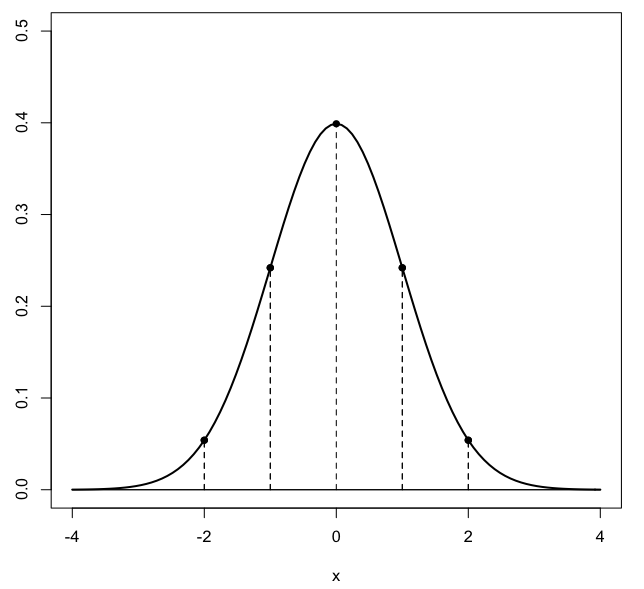
\includegraphics [scale=0.4] {gauss3.png} \end{center}

\title{Gamma function}
\date{}

\begin{document}
\maketitle
\Large

In the chapter on improper integrals, we studied the negative exponential
\[ \int_0^{\infty} e^{-x} \ dx \]
which we formally evaluate at a very large number $a$ and then ask about $a \rightarrow \infty$, but in practice just write
\[ = -e^{-x} \ \bigg |_0^{\infty} \]
\[ = - \ [ \ 0 - 1 \ ] = 1 \]

\subsection*{Euler factorial}

Here is a variant
\[ \int_0^{\infty} x e^{-x} \ dx \]
We can do this by guessing.  Since
\[ [x e^{-x} ]' = e^{-x} - x e^{-x} \]
Rearrange
\[  x e^{-x} = - [x e^{-x} ]' + e^{-x} \]
Integrate both sides and write the bounds
\[ \int_0^{\infty} x e^{-x} \ dx = - x e^{-x} \ \bigg |_0^{\infty} +  \int_0^{\infty} e^{-x} \ dx  \]
For the right-hand side, the second term is just $1$ by the above result
\[ \int_0^{\infty} x e^{-x} \ dx = - x e^{-x} \ \bigg |_0^{\infty} +  1  \]

\subsection*{evaluate a ratio}
So what is
\[ x e^{-x} \ \bigg |_0^{\infty} \]
Which term wins the race?  Write this as a ratio
\[ \frac{x}{e^{x}} \]
At the upper bound we have $\infty/\infty$ so L'Hospital says take the derivative and re-evaluate:
\[ \frac{1}{e^{x}} \]
We have just $e^{-x}$ as $x \rightarrow \infty$ which equals zero.  
At the lower bound
\[ x e^{-x}  = 0 \cdot 1 = 0 \]
Therefore 
\[ x e^{-x} \ \bigg |_0^{\infty} = 0 \]

We proceed to derive a result we will use below.
\[ x^2 e^{-x} \ \bigg |_0^{\infty} = 0 \]
Write the ratio
\[ \frac{x^2}{e^x} \]
we have $\infty/\infty$ so take the derivative, and then take it again, reaching
\[ \frac{2}{e^{x}} \]
We have $2e^{-x}$ as $x \rightarrow \infty$, which equals zero.  
At the lower bound
\[ x^2 e^{-x}  = 0^2 \cdot 1 = 0 \]
since both bounds are zero, the whole thing is zero.
\[ x^2 e^{-x} \ \bigg |_0^{\infty} = 0  \]

Note carefully that $x^n e^{-x}$ is equal to $0$ for any value of $n$ at both the upper bound $x \rightarrow {\infty}$ and at $x = 0$.  Do you see why?

Finishing the problem from the previous section:
\[ \int_0^{\infty} x e^{-x} \ dx = - x e^{-x} \ \bigg |_0^{\infty} +  1 = 1  \]

\subsection*{n = 2}
The next integer is
\[ \int_0^{\infty} x^2 e^{-x} \ dx \]

We do this by IBP.  Let
\[ u = x^2, \ \ \ \ du = 2x \ dx \]
\[ dv = e^{-x} \ dx, \ \ \ \ v = - e^{-x} \]
\[ \int u \ dv = uv - \int v \ du \]
\[ \int_0^{\infty} x^2 e^{-x} \ dx = - x^2 e^{-x} \ \bigg |_0^{\infty} - 2 \int_0^{\infty} - e^{-x} \ x \ dx \]
The first term on the right-hand side is zero, as before.  

\[ \int_0^{\infty} x^2 e^{-x} \ dx =  2 \int_0^{\infty} e^{-x} \ x \ dx = 2 \]

\subsection*{higher values of n}
\[ \int_0^{\infty} x^n e^{-x} \ dx \]
Use IBP
\[ u = x^n, \ \ \ \ du = nx^{n-1}\ dx \]
\[ dv = e^{-x} \ dx, \ \ \ \ v = - e^{-x} \]
\[ \int u \ dv = uv - \int v \ du \]

\[ \int_0^{\infty} x^n e^{-x} \ dx = - x^n e^{-x} \ \bigg |_0^{\infty} + n \int_0^{\infty} x^{n-1} e^{-x} \ dx\]
but that first term on the right-hand side is zero so
\[ \int_0^{\infty} x^n e^{-x} \ dx = n \int_0^{\infty} x^{n-1} e^{-x} \ dx\]
For $n=3$
\[ \int_0^{\infty} x^3 e^{-x} \ dx = 3 \int_0^{\infty} x^{2} e^{-x} \ dx = 3 \cdot 2 \]
For $n=4$
\[ \int_0^{\infty} x^4 e^{-x} \ dx = 4 \int_0^{\infty} x^{3} e^{-x} \ dx = 4 \cdot 3 \cdot 2 = 4! \]
The general result is
\[ \int _0^{\infty}x^n e^{-x} \ dx =  n \int_0^{\infty} x^{n-1} e^{-x} \ dx = n! \]

\subsection*{Gamma function}
The generalized function is usually written with $t$ as the variable and $x$ as the power
\[ \int_0^{\infty} t^x e^{-t} \ dt = x!  \]
The gamma function ($\Gamma$) is defined to be
\[ \Gamma(x + 1) = \int_0^{\infty} t^x e^{-t} \ dt = x! \]

The reason for this shift (using $x + 1$ in the function definition) is given here:

\url{http://www.sosmath.com/calculus/improper/gamma/gamma.html}

It has to do with the domain of $x$ for which the function is defined.  The original domain is $(-1, \infty)$, but after the shift it is $(0, \infty)$.

\subsection*{properties}

As a result of the definition in the previous section
\[ \Gamma(x + 1) = x \Gamma(x) = x! \]
so 
\[ \Gamma(x) = (x-1)! \]
\[ \Gamma(1) = \int_0^{\infty} t^0 e^{-t} \ dt = 1 \]

So far we have only considered $\Gamma(x)$ for $x \in \mathbb{N}$, but in fact the formula works for fractional $x = p/q$ which means that we can write $\Gamma (1/2)$ and actually evaluate it.

\[ \Gamma(\frac{1}{2}) = \int _0^{\infty} x^{-1/2} e^{-x} \ dx \]
\[ = \int _0^{\infty} \frac{e^{-x}}{\sqrt{x}} \ dx \]
Substitute $x = t^2$, then $dx = 2 t \ dt$ and
\[ \int _0^{\infty} \frac{e^{-t^2}}{t} 2t \ dt \]
\[ = 2 \int _0^{\infty} e^{-t^2} \ dt \]
We solved this integral in the chapter on the normal distribution:
\[ \int_{-\infty}^{\infty} e^{-kx^2} \ dx = \sqrt{\frac{\pi}{k}} \]
Here, $k = 1$ so
\[ \int_{-\infty}^{\infty} e^{-x^2} \ dx = \sqrt{\pi} \]
This is an even function so
\[ \int_0^{\infty} e^{-x^2} \ dx = \frac{\sqrt{\pi}}{2} \]
which means the value of the integral given above is just $\sqrt{\pi}$.
\[ \Gamma(\frac{1}{2}) = \sqrt{\pi} \]

Some people like to write things like $(-1/2)!$ at this point, and while others prefer to say that the Gamma function gives the same result as the factorial for the positive integers, but also is also defined for rational numbers.

Since
\[ \Gamma(x + 1) = x \Gamma(x) \]
\[ \Gamma(\frac{3}{2}) = \frac{1}{2} \cdot \Gamma(\frac{1}{2}) = \frac{\sqrt{\pi}}{2} \]
\[ \Gamma(\frac{5}{2}) = \frac{3}{2} \cdot \Gamma(\frac{3}{2}) = \frac{3}{2} \cdot \frac{\sqrt{\pi}}{2} \]

Here's a quote from 

\url{http://mhtlab.uwaterloo.ca/courses/me755/web_chap1.pdf}

\begin{quote}The gamma function is one of the most widely used special functions encountered in advanced mathematics because it appears in almost every integral or series representation of other advanced mathematical functions.\end{quote}

\subsection*{historical aside}
In \emph{An Imaginary Tale}, Nahin says that Wallis "knew" the particular result given above, namely $\Gamma(1/2) = \sqrt{\pi}$, although of course the notation $\Gamma$ was only introduced later.

Like many people in the years just before Newton, he was investigating the area under certain curves.  One family of curves Wallis looked at is 
\[ f(x) = (x - x^2)^n \]

He found that the value of the integral is given by
\[ \int_0^1 (x - x^2)^n \ dx = \frac{(n!)^2}{(2n + 1)!} \]

I used the program described in the chapter on Numerical Integration

\url{https://gist.github.com/telliott99/5a1190217a130c7ee01dee17ea483f7b}

 to evaluate the integral for $n=2,3,4$ and obtained:
\[ n=2, \ \ \ 0.033333333625 \]
\[ n=3, \ \ \ 0.00714285699705 \]
\[ n=4, \ \ \ 0.00158730158727 \]

Very similar values are obtained by evaluating
\[ \frac{(n!)^2}{(2n + 1)! } \]
e.g with $n=4$
\[ \frac{24^2}{362880} =  0.00158730 \]

Here is the connection to $1/2$.  A circle of unit \emph{diameter} placed with its center at $(1/2,0)$ has the equation:
\[ (x - \frac{1}{2})^2 + y^2 = \frac{1}{4} \]
\[ y^2 =  \frac{1}{4} - x^2 + x - \frac{1}{4} = x - x^2 \]
\[ y = \sqrt{x - x^2} = (x - x^2)^{1/2} \]
The area above the $x$-axis is
\[ \int_0^1 \sqrt{x - x^2} \ dx \]
We know the area under this curve from the geometry of the circle, it is just one-half of $\pi/4 = \pi/8$.

Plugging the power of $n = 1/2$ into the factorial formula:
\[ \frac{(n!)^2}{(2n + 1)!} \]
\[ \frac{((1/2)!)^2}{2} = \frac{\pi}{8} \]
\[ ((1/2)!)^2 = \frac{\pi}{4} \]
\[ (1/2)! = \frac{\sqrt{\pi}}{2} \]

How about that!

\subsection*{Beta function}
The Gamma function is related to the Beta function, which has wide application in probability.

The beta distribution is
\[ f(x) = x^{p - 1} (1 - x)^{q - 1} \]

The beta function is defined as follows:
\[ B (p,q) = \int_0^1 x^{p - 1} (1 - x)^{q - 1} \ dx, \ \ \ p > 0, q > 0 \]

You may recognize this expression as being related to the binomial distribution.  The value obtained from the integral can be used to normalize the distribution so that it is a proper pdf.

Here is a great explanation:

\url{http://varianceexplained.org/statistics/beta_distribution_and_baseball}

The example is batting averages in baseball.

\begin{quote}Given our batting average problem, which can be represented with a binomial distribution (a series of successes and failures), the best way to represent these prior expectations (what we in statistics just call a prior) is with the beta distribution ...

We expect that the player's season-long batting average will be most likely around .27, but that it could reasonably range from .21 to .35. This can be represented with a beta distribution with parameters $\alpha=81$ and $\beta=219$\end{quote}

We let 
\[ f(x) = x^{p - 1} (1 - x)^{q - 1} \]
with $p=81$ and $q=219$.  

Here is a Python script to plot the distribution:

\url{https://gist.github.com/telliott99/74bb7a47adb692b60fcbf00dd9829901}

\begin{center} 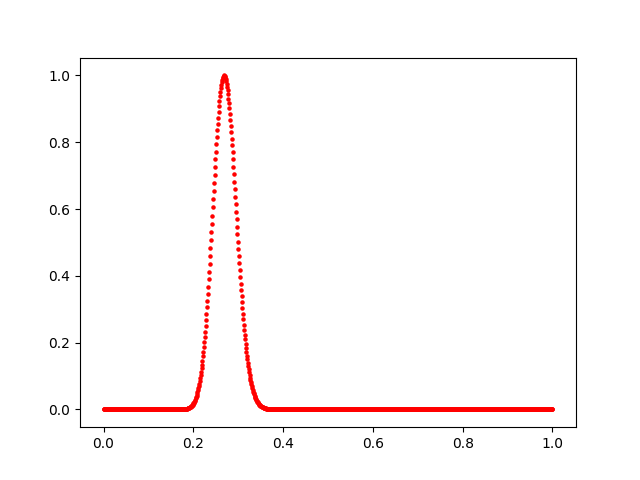
\includegraphics [scale=0.5] {beta_example.png} \end{center}

The mean of the beta distribution is simply $p/p+q = 81/(81 + 219) = 0.27$.  The magnitudes of $p$ and $q$ determine the width of the peak, chosen here to approximate $[0.21,0.35]$.  Nearly all the density for historical batting averages lies in this range.

The beta function we defined is the integral of this pdf over the range $[0,1]$.  We'll see that this integral can be expressed in terms of the Gamma function, and this makes it easy to calculate.

\[ B(p,q) = \frac{\Gamma(p) \ \Gamma(q)}{\Gamma (p + q)} \]

\subsection*{derivation}

\[ B (p,q) = \int_0^1 x^{p - 1} (1 - x)^{q - 1} \ dx, \ \ \ p > 0, q > 0 \]

If we make a trigonometric substitution $x = \sin^2 \theta$, we have
\[ B (p,q) = \int (\sin^2 \theta)^{p - 1} \ (\cos^2 \theta)^{q - 1} \ 2 \sin \theta \cos \theta \ d \theta \]
\[  = 2 \int (\sin \theta)^{2p - 1} \ (\cos \theta)^{2q - 1} \ d \theta \]

At the lower bound $x = 0, \theta = 0$, and at the upper bound $x = 1, \theta = \pi/2$ so
\[  B (p,q) = 2 \int_0^{\pi/2} (\sin \theta)^{2p - 1} \ (\cos \theta)^{2q - 1} \ d \theta \]

\subsection*{Relationship to the Gamma function}
Recall that
\[ \Gamma(p) = \int_0^{\infty} t^{p-1} e^{-t} \ dt \]
Substitute $t = x^2$, $dt = 2x \ dx$ so
\[ \Gamma(p) = 2 \int_0^{\infty} x^{2(p-1)} x \ e^{-x^2} \ dx \]
\[ = 2 \int_0^{\infty} x^{2p-1} \ e^{-x^2} \ dx \]

$x$ and $y$ are both \emph{dummy} variables in what follows so we can write
\[ \Gamma(q) = 2 \int_0^{\infty} y^{2q-1} \ e^{-y^2} \ dy \]

Multiplying
\[ \Gamma(p) \ \Gamma(q) = 4 \int_0^{\infty} x^{2p-1} \ e^{-x^2} \ dx \  \int_0^{\infty} y^{2q-1} \ e^{-y^2} \ dy \]
\[ = 4 \int_0^{\infty} \int_0^{\infty} x^{2p-1} y^{2q-1} \ e^{-x^2} \ e^{-y^2} \ dx \ dy \]

$x$ and $y$ are independent, so we can think of this as a double integral in the plane and switch to polar coordinates with $e^{-x^2} \cdot e^{-y^2}  = e^{-(x^2 + y^2)} = e^{-r^2}$
\[ \Gamma(p) \ \Gamma(q) = 4  \int_0^{\pi/2} \int_0^{\infty} (r \sin \theta)^{2p-1} (r \cos \theta)^{2q-1} \ e^{-r^2}  \ r \ dr \ d \theta  \]
The bounds on $\theta$ are the first quadrant of the plane, the same quadrant where the first double integral was taken.

The $r$ part and the $\theta$ part are independent so we have two components (split the factor of $4$):
\[ I_r = 2 \int_0^{\infty} r^{2p + 2q - 1} e^{-r^2} \ dr  \]
compare with this expression from above:
\[ \Gamma(p) = 2 \int_0^{\infty} x^{2p-1} \ e^{-x^2} \ dx \]
We see that 
\[ I_r = \Gamma (p + q) \]

For the $\theta$ part of the integral
\[ I_{\theta} = 2 \int_0^{\pi/2}  (\sin \theta)^{2p-1} (\cos \theta)^{2q-1} \ d \theta  \]
compare with the definition of the beta function
\[  B (p,q) = 2 \int_0^{\pi/2} (\sin \theta)^{2p - 1} \ (\cos \theta)^{2q - 1} \ d \theta \]
We see that these are identical 
\[ I_{\theta} = B(p,q) \]

Combining the results:
\[ \Gamma(p) \ \Gamma(q) = I_r \ I_{\theta} = \Gamma (p + q) \ B(p,q) \]
and so
\[ B(p,q) = \frac{\Gamma(p) \ \Gamma(q)}{\Gamma (p + q)} \]
\[ = \int_0^1 x^{p - 1} (1 - x)^{q - 1} \ dx , \ \ \ p > 0, q > 0 \]

\subsection*{application}

If you want to see an application to Bayesian probability look at this great post:

\url{https://alexanderetz.com/2015/07/25/understanding-bayes-updating-priors-via-the-likelihood/}

The basic idea in Bayes is that we have some current information about the process of interest (called the prior), and that we update probabilities of whatever we're trying to estimate based on new data (called the likelihood).  In the example, we're trying to estimate the probability of success of a 3-point shot in basketball.

Mathematically, the update happens by multiplying the likelihood times the prior.  These are two integrals.  The multiplication is easy to do if the two integrals are of the same type (called conjugate distributions), for example, if they are both beta functions.  That is natural when the data is of this type, from a series of Bernoulli trials.




\end{document}